\documentclass{article}
\linespread{1.3}
\usepackage[margin=50pt]{geometry}
\usepackage{amsmath, amsthm, amssymb, amsthm, tikz, fancyhdr}
\pagestyle{fancy}
\renewcommand{\headrulewidth}{0pt}
\newcommand{\changefont}{\fontsize{15}{15}\selectfont}

\fancypagestyle{firstpageheader}
{
  \fancyhead[R]{\changefont Michael Huang \\ CFRM 415 \\ Midterm}
}

\begin{document}

\thispagestyle{firstpageheader}

\framebox[1.1\width]{\textbf{answer}}

\section*{1.}

{\Large 

\subsection*{(a)}

$\mu^T = 
\begin{bmatrix}
  0.3 & 0.6 & 0.7
\end{bmatrix}$ \\
$ \Sigma = 
\begin{bmatrix}
2.5 & 1.2 & 0.3 \\
1.2 & 3.1 & 1.3 \\
0.3 & 1.3 & 2.4
\end{bmatrix}$ \\ 

We optimize by minimizing $\frac{1}{2} \omega^T \Sigma \omega$ with $\omega^T 1 = 1$, and doing the Lagrangian, we find that \\
$\widehat{\omega} = \frac{\Sigma^{-1}1}{1^T\Sigma^{-1}1}$ \\
$\widehat{\omega} = 
\begin{bmatrix}
  0.33604008 \\ 
  0.04578438 \\ 
  0.34986178 \\ 
\end{bmatrix} 
\div
\begin{bmatrix}
  0.73168625
\end{bmatrix}$ \\
$\widehat{\omega} = 
\begin{bmatrix}
  0.459268 \\ 
  0.06257379 \\
  0.47815821
\end{bmatrix}$ \\
The optimal weights are therefore \framebox[1.1\width]{\textbf{0.459268, 0.06257379, 0.47815821}} \\ \\ 
We simply multiply to get the expected annual return: \\
$= \widehat{\omega}^T \cdot  \mu$ \\
$=
\begin{bmatrix}
  0.51003542
\end{bmatrix}$ \\
The expected annual return is therefore \framebox[1.1\width]{\textbf{0.51003542}} \\ \\
To find the portfolio volatility, we find the square root of the variance: \\
$= \sqrt{\widehat{\omega}^T \Sigma \widehat{\omega}}$ \\
$= \sqrt{\frac{1}{1^T \Sigma^{-1} 1}}$ \\
$= \sqrt{1.36670602}$ \\
$= 1.16906203$ \\
The portfolio volatility is therefore \framebox[1.1\width]{\textbf{1.16906203}}

\subsection*{(b)}

Let $\gamma > 0$ be an investor’s risk tolerance. Calculate the mean and variance of the portfolio returns generated by the weights optimizing the general Markowitz optimization problem. Note: You do not need to compute the optimal weights for this case. \\ \\

% Show previous algebra
We define $A = 1^T \Sigma^{-1} 1$, $B = \mu^T \Sigma^{-1} 1$, $C = \mu^T \Sigma^{-1} \mu$. We can calculate these values as scalars, and redefine them as $A = 0.73168625$, $B = 0.3731859$, $C = 0.23130615$.
We know that the portfolio mean can be represented as \\
$\mu = \frac{B}{A} + \frac{1}{\gamma} \frac{AC - B^2}{A}$ \\
$\mu = \frac{0.3731859}{0.73168625} + \frac{1}{\gamma} \frac{0.73168625 \cdot 0.23130615 - 0.3731859^2}{0.73168625}$ \\
$\mu = 0.51003541477 + \frac{1}{\gamma} \frac{0.16924352949 - 0.13926771595}{0.73168625}$ \\
$\mu = 0.51003541477 + \frac{0.04096812471}{\gamma}$ \\
The portfolio mean is therefore \framebox[1.1\width]{\textbf{$0.51003541477 + \frac{0.04096812471}{\gamma}$}} \\ \\
We know that the portfolio variance can be represented as \\
$\sigma^2 = \frac{1}{A} + \frac{1}{\gamma^2} \frac{AC - B^2}{A}$ \\
$\sigma^2 = \frac{1}{0.73168625} + \frac{1}{\gamma^2} \frac{0.73168625 \cdot 0.23130615 - 0.13926771595}{0.73168625}$ \\
$\sigma^2 = 1.36670601641 + \frac{1}{\gamma^2} \frac{0.16924352949 - 0.13926771595}{0.73168625}$ \\
$\sigma^2 = 1.36670601641 + \frac{0.04096812471}{\gamma^2}$ \\
The portfolio variance is therefore \framebox[1.1\width]{\textbf{$1.36670601641 + \frac{0.04096812471}{\gamma^2}$}}

}

\section*{2.}

{\Large

Let $R_i$ and $R_j$ be random variables representing annual excess returns on securities $i$ and $j$ in the total market, under the assumptions of the CAPM. \\

\subsection*{(a)}

Write the regression equation for $R_i$, including the statistical conditions on the error terms, and identify the terms representing the systematic and idiosyncratic risks. \\

By CAPM, we know that \\
$r_i = \alpha_i + r_f + \beta_i(r_M - r_f) + \epsilon_i$ \\ 
$R_i = \alpha_i + \beta_i (r_M - r_f) + \epsilon_i$ \\
$R_i = \alpha_i + \beta_i (R_M) + \epsilon_i$ \\
with $\epsilon_i$ statistically defined with expectation 0, and variance $\sigma_i^2$ \\ \\
We have that $\epsilon_i$ is the idiosyncratic or non-systematic risk since it is directly associated with security $i$, while $\beta_i (R_M)$ is the systematic risk as it is only correlated with the market.
% $\beta_i = \frac{Cov(r_i, r_M)}{\sigma_M^2}$

\subsection*{(b)}

We aim to show that $\sigma_{ij} = \beta_i \beta_j \sigma_M^2$, or that $Cov(R_i, R_j) = \beta_i \beta_j \sigma_M^2$. \\
By CAPM, we know that \\
$R_i = \alpha_i + \beta_i (R_M) + \epsilon_i$ \\
$R_j = \alpha_j + \beta_j (R_M) + \epsilon_j$ \\
We can start with $Cov(R_i, R_j)$ \\ 
$= Cov (\alpha_i + \beta_i (R_M) + \epsilon_i, \alpha_j + \beta_j (R_M) + \epsilon_j)$ \\
$= Cov(\beta_i (R_M) + \epsilon_i, \beta_j (R_M) + \epsilon_j)$ \hfill Constants don't affect covariance \\ 
$= Cov(\beta_i (R_M), \epsilon_j) + Cov(\beta_i (R_M), \beta_j (R_M)) + Cov(\beta_j (R_M), \epsilon_i) + Cov(\epsilon_i, \epsilon_j)$ By Hint \\
$= 0 + Cov(\beta_i (R_M), \beta_j (R_M)) + 0 + 0$ \hfill $\epsilon$ is idiosyncratic/specific to security $i/j$ \\ 
$= Cov(\beta_i (R_M), \beta_j (R_M))$ \\
$= \beta_i \beta_j Cov((R_M), (R_M))$ \hfill Definition of covariance \\
$= \beta_i \beta_j Var(R_M)$ \hfill Definition of variance \\
$= \beta_i \beta_j \sigma^2_M$ \\
as we hoped to show.


% As stated previously, by CAPM, we know that $\beta = \frac{Cov(r_p, r_M)}{\sigma_M^2}$

}

\section*{3.}
{\Large 

Suppose that the risk-free rate of interest is 0.07, and the expected rate of return on the market portfolio is 0.14. The volatility (standard deviation) of the market portfolio is 0.12.

We are given that $r_f = 0.07, r_M = 0.14, \sigma_M = 0.12$.

\subsection*{(a)}

\begin{figure}[h]
  \centering
  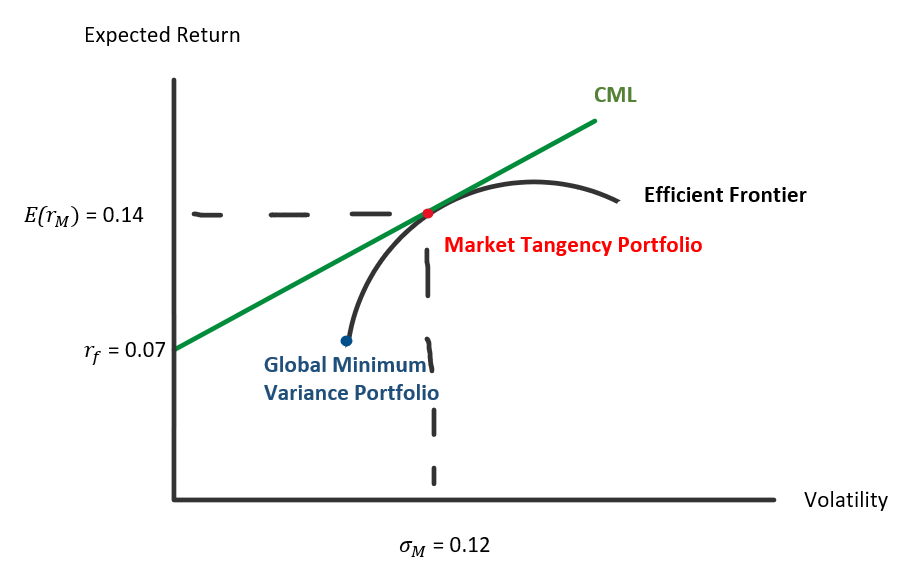
\includegraphics[width=120mm]{./3a.png}
\end{figure}

\subsection*{(b)}

Suppose that of our entire portfolio, we put $y$ towards the market portfolio:
$0.11 = 0.07(1-y) + 0.14(y)$ \\ 
$0.11 = 0.07 - 0.07y + 0.14y$ \\ 
$0.04 = 0.07y$ \\ 
\framebox[1.1\width]{\textbf{$y = \frac{4}{7}$ towards the risky asset, and $ 1 - y = \frac{3}{7}$ towards the risk-free asset.}} 


\subsection*{(c)}

We can find the optimal way to invest using the CML which is graphed according to CAPM. A way to do this is by using the equation for the CML. Given two known points (0, 0.07) and (0.12, 0.14), we know its slope to be $\frac{0.14-0.07}{0.12 - 0} = \frac{0.07}{0.12} = \frac{7}{12}$, and the y-intercept to be 0.07. This gives us the equation $0.11 = \frac{7}{12}\sigma + 0.07$. We can therefore solve for the level of volatility for an expected return of 0.11: \\
$0.11 = \frac{7}{12}\sigma + 0.07$ \\
$0.04 = \frac{7}{12}\sigma$ \\
$\frac{1}{25} \cdot \frac{12}{7} = \sigma$ \\
$\frac{12}{175} = \sigma$ \\
$\sigma = $ \framebox[1.1\width]{\textbf{$\sim$ 0.06857}}

}

\section*{4.}
{\Large 

You enter into a one-year payer swap that pays cashflows semiannually. The value date (today, 2021.05.06) is the first reset date, and assume the notional value is 1 (to keep it simple), until you get to part (e).

\subsection*{(a)}
Assuming that a reset date that falls on a weekend or holiday is rolled to the next business day, write out the reset and payment dates for the swap; notate them with 𝑇0,𝑇1,𝑇2 in your answer.

\subsection*{(b)}

Assuming an Actual/360 day-count convention, calculate and write out the day-count adjusted year fractions 𝜏1, 𝜏2 , and 𝜏(𝑇0,𝑇2). You may use a tool like R/lubridate, Excel, etc to calculate the number of days between the dates and just indicate these results in your calculations. You will need the results in subsequent sections.

\subsection*{(c)}

}

\section*{5.}
{\Large 



}


\end{document}